
\section{Seismicity Parameters}
\label{sec:params}

Following the general approach described in the previous sections and using the information collected about the seismic catalog and its completeness, we computed the seismicity parameters $a$ and $b$, and the maximum magnitude $M_{\max}$ using the seismic hazard assessment software HA3, version 3 \citep{Kijko_2004_HA3}. This software implements the procedures developed by \citet{Kijko_1989_BSSA, Kijko_1992_BSSA}, and subsequent updates by \citet{Kijko_2004_PAG}. HA3 is widely used for this type of computations and is regarded as a reliable tool in seismic hazard analysis \citep[see, for instance,][]{Karimiparidari2013, Khodaverdian_2016_BSSA}.

The $a$-value is estimated based on the completeness year, the correlation distance, and the number of events per grid cell. We assume magnitude increments of $\Delta M = 0.1$, count events with magnitude $M_w > 3$, and smooth the number of events for each cell. This means each cell has a different $a$-value and thus the result is variable throughout our region of interest. On the other hand, we consider the $b$-value and $M_{\max}$ to be constant within each of the seismic zones in our study area. We compute $b$ and $M_{\max}$ using HA3 and the information from the catalog. \myrevision{ Regional maximum magnitude is estimated according to \citet{Kijko_1989_BSSA} method. Magnitude errors are distributed normally and $\beta$ and $\lambda$ are calculated simultaneously.  We divide the} catalog in five sub-catalogs: one incomplete catalog for the prehistorical period before 1000, one incomplete catalog for the historical period between 1000 and 1799, one complete catalog for the early instrumental period between 1800 and 1899, and two complete catalogs for the instrumental periods between 1900 and 1999, and between 2000 and 2015. In this process we use the values of $M_c$ shown in Table \ref{tab:completeness}. 

We obtain $b$ and $M_{\max}$ for two different models. In the first model we obtain these parameters independently for each one of the five seismic zones influencing the hazard in northern Iran. We call this the \textit{R Model}. In it we obtain distinct values of $b$ and $M_{\max}$ for the main northern seismic zones of Azerbaijan, Alborz, and Kopeh Dagh, as well as for the Zagros and Central-East seismic zones contributing to our region of interest (see Fig.~\ref{fig:iran} for reference). In the second model we consider the whole study area as a uniform seismic zone. We call it the \textit{U Model}. Admittedly, this assumption is somewhat unrealistic if considered from the point of view that different seismic zones \myrevision{may have different values of $b$ and $M_{max}$}. However, as it will be seen in the Results and Analysis section, computing results for this uniform model was useful because it allowed us to find a combination model computation of hazard in the region of interest as a means to \myrevision{account for} epistemic uncertainty. Table \ref{tab:params} shows the parameters $b$ and $M_{\max}$ obtained with HA3 for the five seismic zones in the R model and the corresponding ones for the U model, along with the observed maximum magnitude, $M_{\max}^{\mathrm{obs}}$; and Fig.~\ref{fig:annualp} shows the annual probability of exceedance as a function of earthquake magnitude.
\myrevision{
\begin{table}%[t]
    \centering
    \caption{Seismicity parameters $b$ and $M_{\max}$ computed for the seismic zones in our region of interest and the reference uniform seismicity model along with the observed maximum magnitude, $M_{\max}^{\mathrm{obs}}$.}
    \begin{tabular}{@{\hspace{0.2ex}}lccc@{\hspace{0.2ex}}}
        \cline{2-4}                                                                         \\[-1.6ex]
                        & $b$-value         & $M_{\max}$        & $M_{\max}^{\mathrm{obs}}$ \\[0.6ex]
        \hline                                                                              \\[-1.6ex]
        Azerbaijan      & 1.15 $\pm$ 0.03   & 7.80 $\pm$ 0.50   & 7.7                       \\
        Alborz          & 0.97 $\pm$ 0.02   & 7.82 $\pm$ 0.52   & 7.8                       \\
        Kopeh Dagh      & 0.93 $\pm$ 0.03   & 7.74 $\pm$ 0.29   & 7.6                       \\
        Zagros          & 1.05 $\pm$ 0.02   & 7.48 $\pm$ 0.26   & 7.4                       \\
        Central-East    & 0.99 $\pm$ 0.02   & 7.80 $\pm$ 0.37   & 7.6                       \\
        Uniform Model   & 0.98 $\pm$ 0.01   & 7.80 $\pm$ 0.28   & 7.8                       \\[0.5ex]
        \hline 
    \end{tabular}
    \label{tab:params} 
\end{table}
}
\begin{figure*}[t]
    \centering
    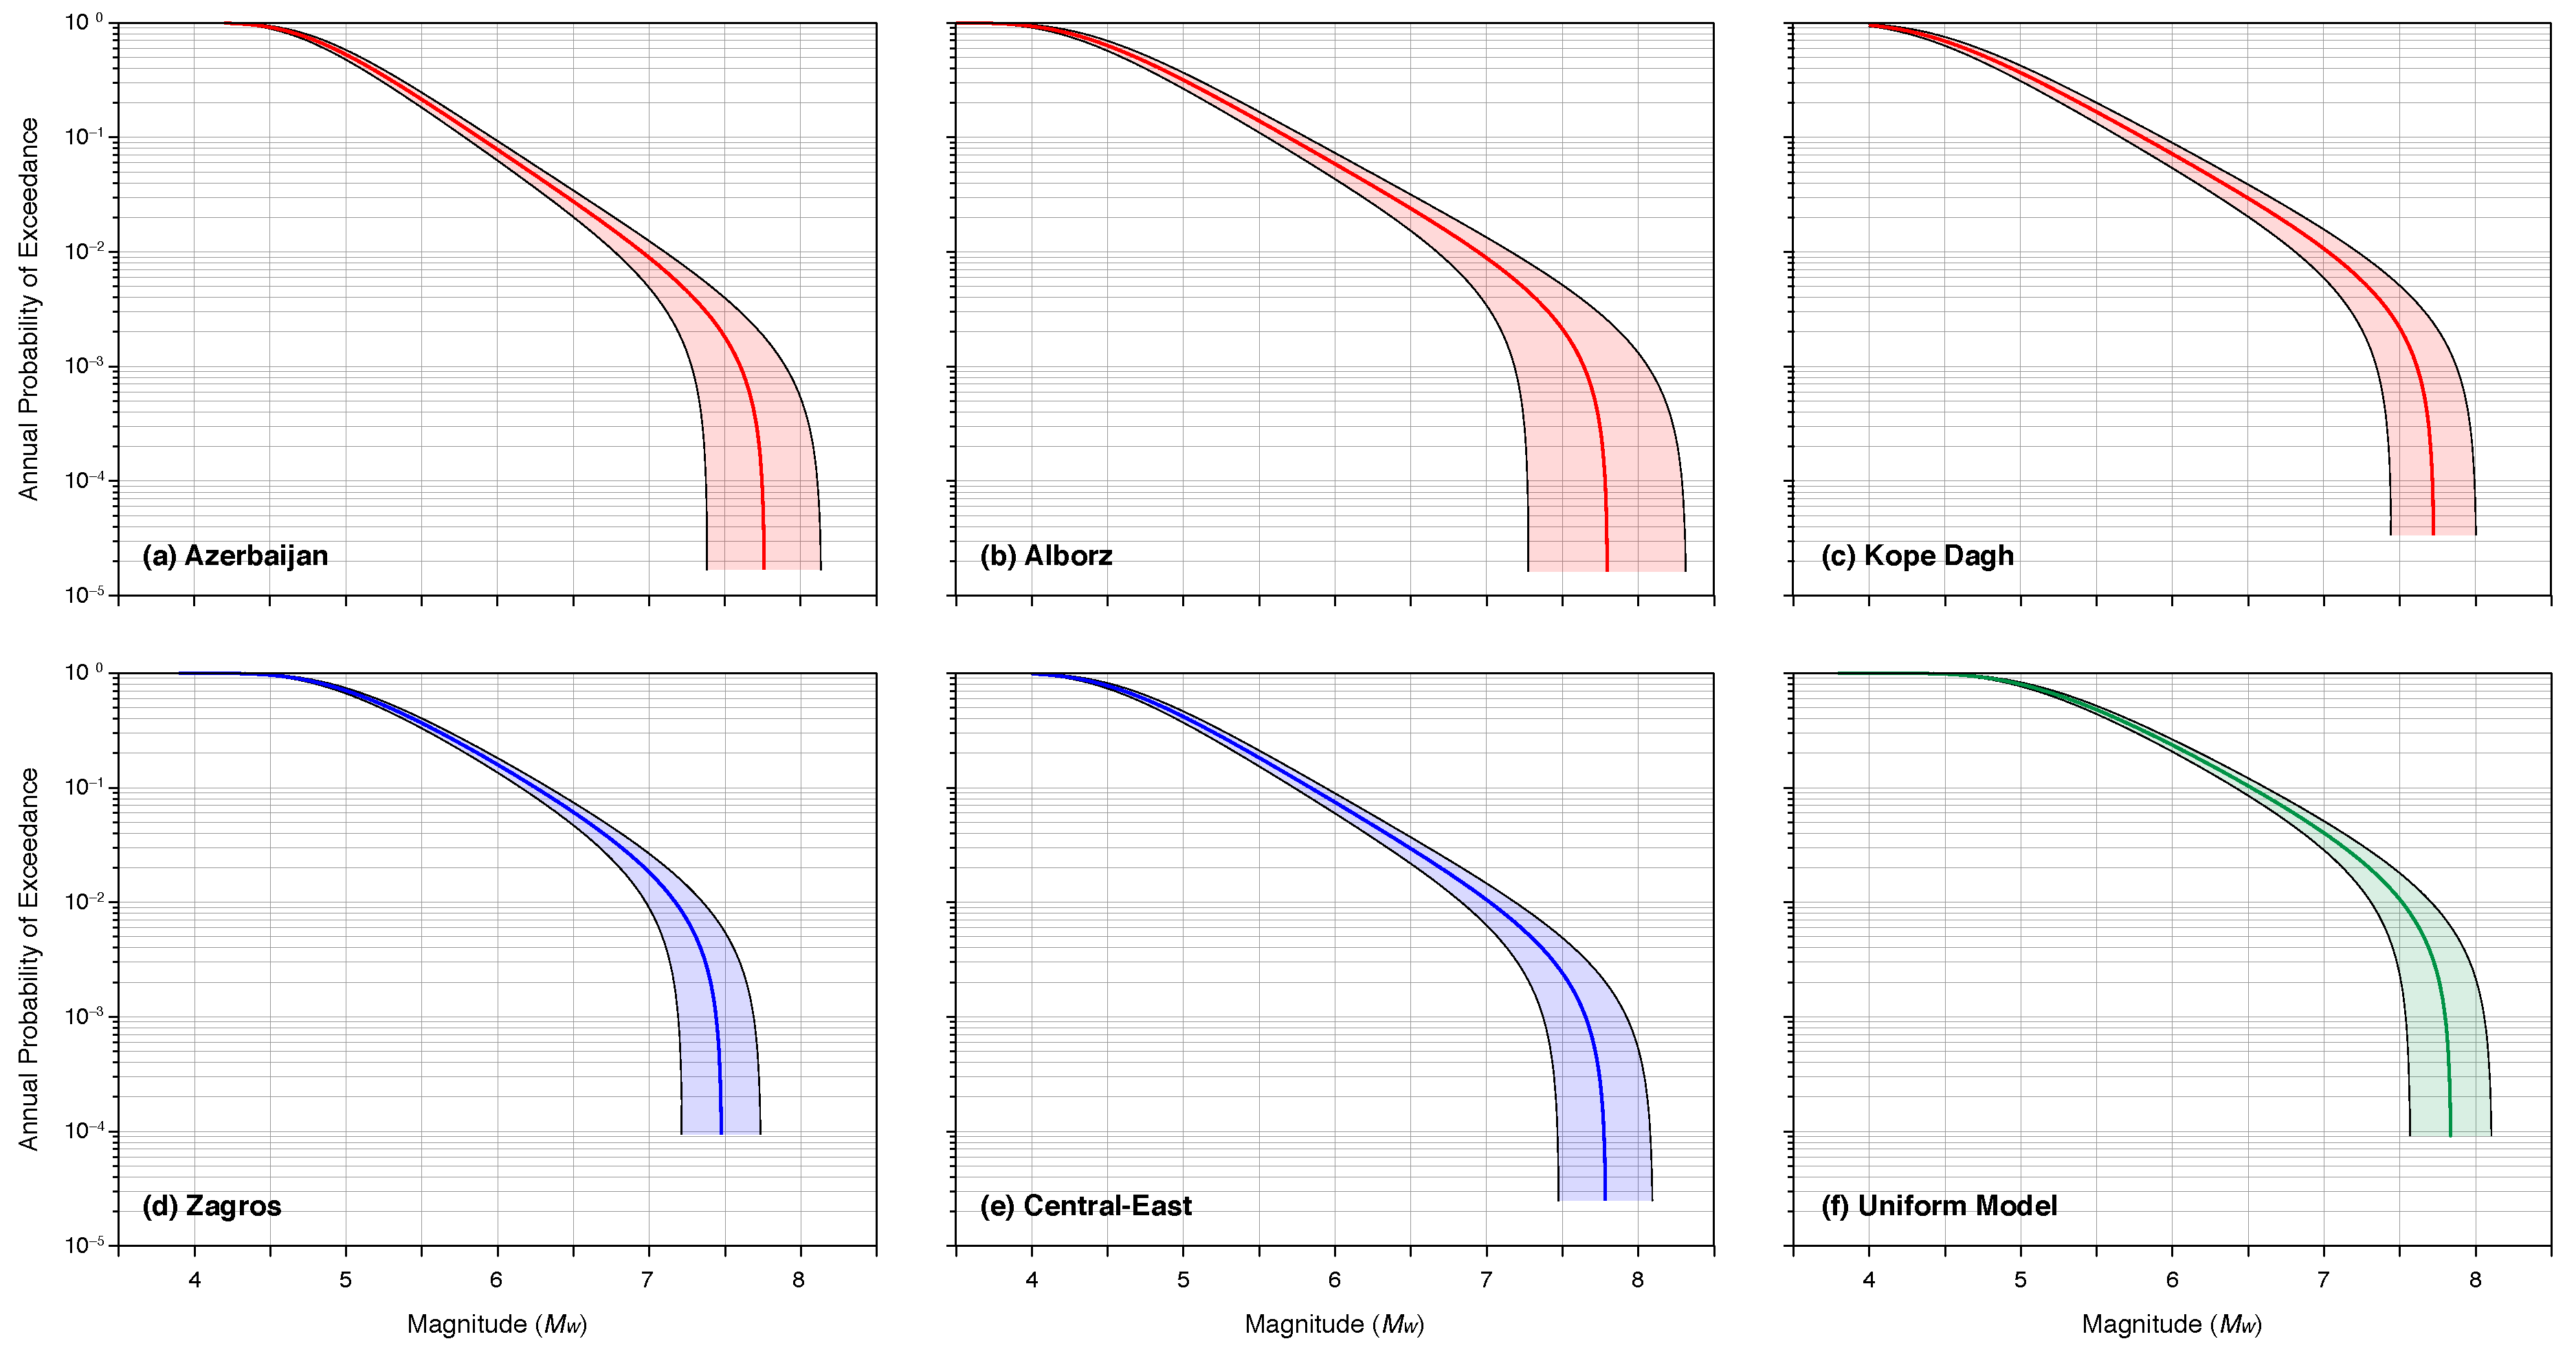
\includegraphics[width=\textwidth]{figures/pdf/figure-07} 
    \caption{Annual probability of exceedance as a function of earthquake magnitude for the seismic zones in the region of interest. The three curves in red correspond to those seismic zones completely considered within the study area, whereas the ones in blue are the two additional contributing zones from the rest of the country. The last curve in green corresponds to the complete region of interest, here referred to as the uniform model. The shaded range indicates the models' $\pm 1$ standard deviation.}
    \label{fig:annualp}
\end{figure*}

